\chapter{Optization of Hyperparameters of Motion Prediction}

\section{Definition of the Prediction Error}

\begin{figure}[htbp]
\centering
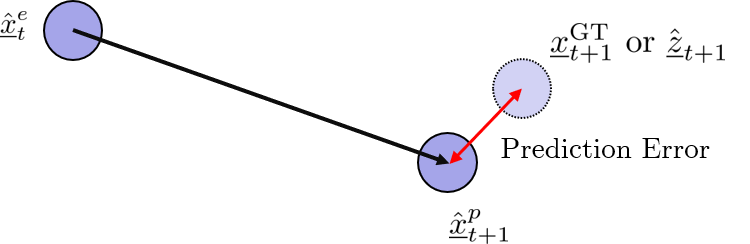
\includegraphics[width=0.9\textwidth]{figures/KF/prediction error.png}
\caption{Definition of the prediction error}
\label{prediction error}
\end{figure}

The prediction error gives a metric for the accuracy of the prediction. The prediction error for each track is defined as the distance between the prediction and the new measurements for real datasets, or the ground truth value for DEM datasets on the last timestep of the track. For the whole dataset the error is defined as the summation of the prediction error of all tracks. 


\section{Effect of the Hyperparameter}

\subsection{seperated}

First, each hyperparameter is tested with the grid-search-like method, in order to find the effect of each hyperparameter.

Some plots like this

\begin{figure}[htbp]
\centering
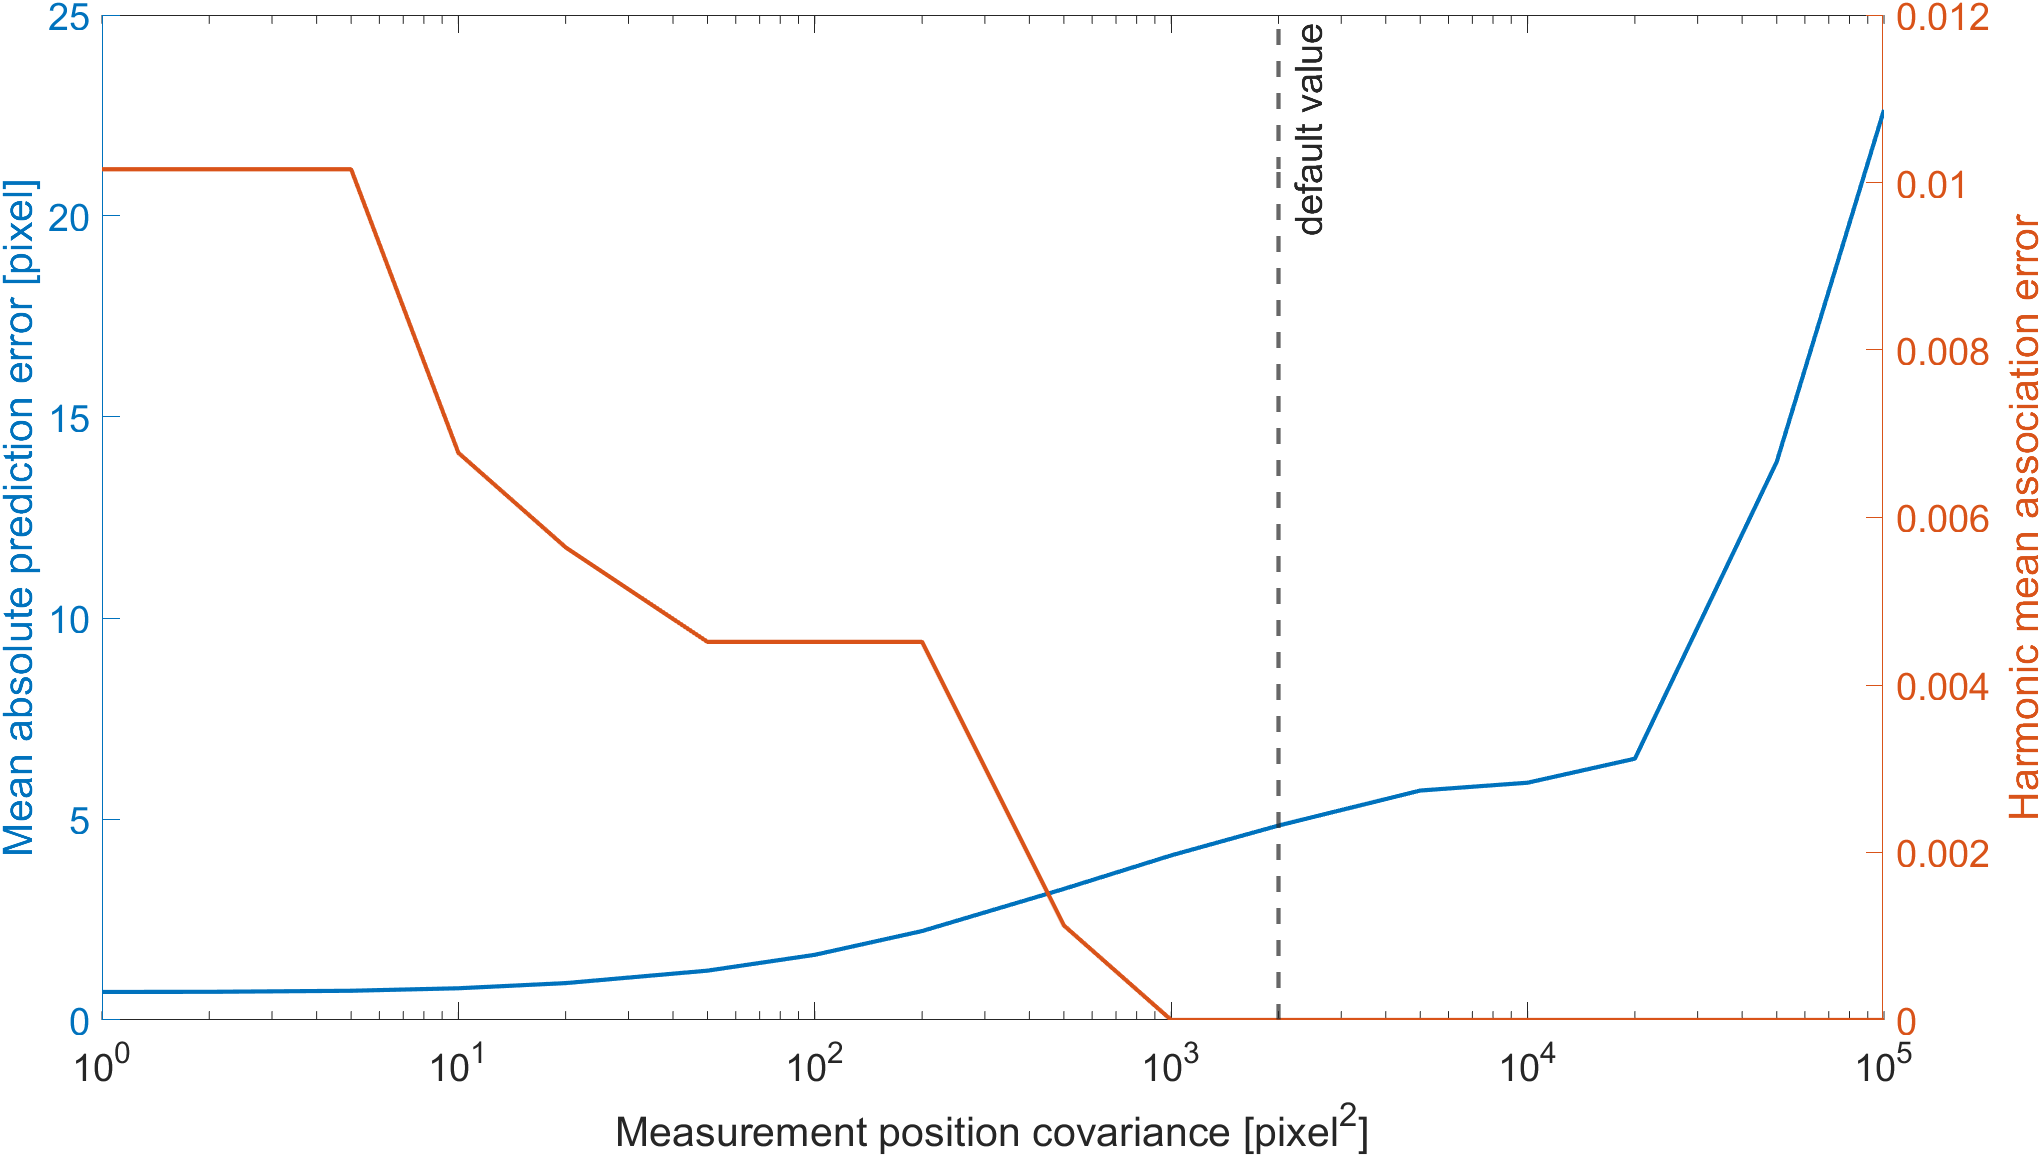
\includegraphics[width=0.9\textwidth]{figures/KF/meacov.png}
\caption{The effect of the measurement position covariance.}
\label{meacov}
\end{figure}

There should be the plots from all hyperparameters for Kalman filter in CV and CVA model. (or only post some of plots here and put others into the appendix)

From the the plots the effect of each hyperparameter is clear. We can also find the measurement and prediction position covariance have the most significant effect on the final tracking error. It should be a important result which is used in the part of optimization. 

\subsection{together}

Some plot like this.

\begin{figure}[htbp]
\centering
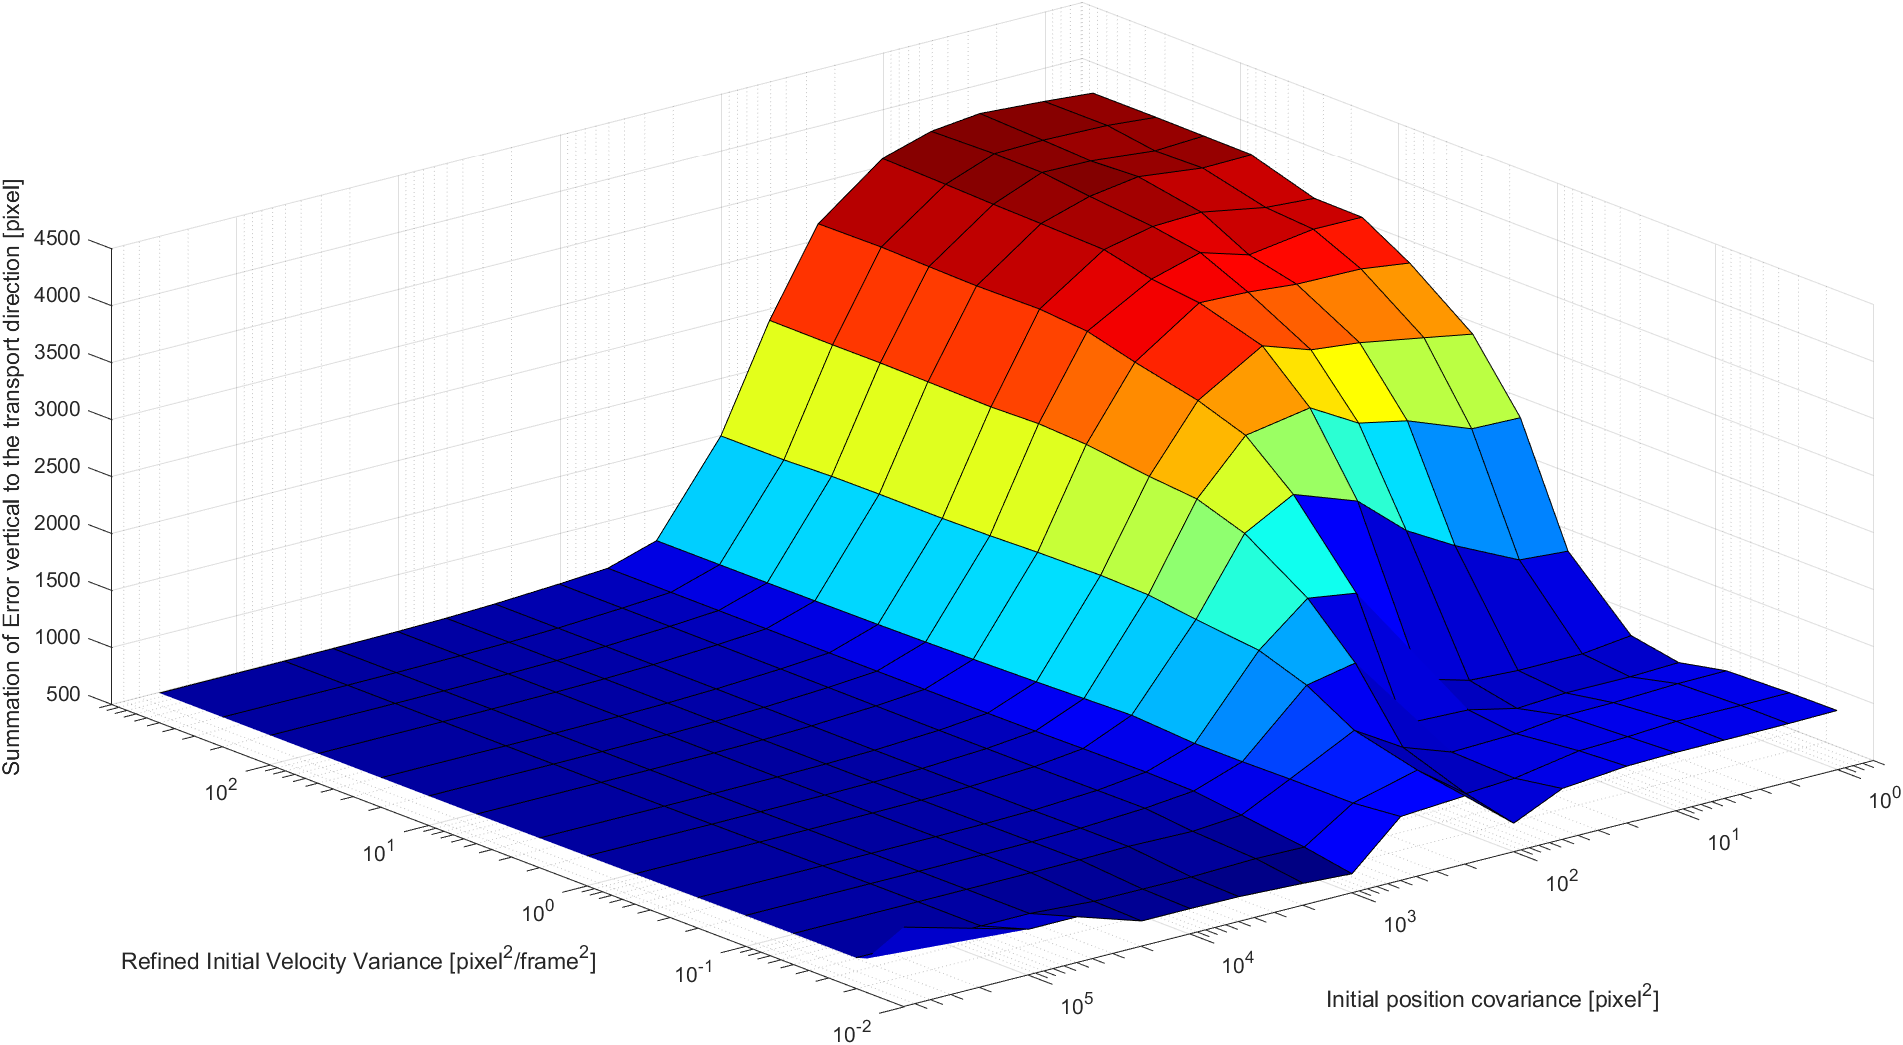
\includegraphics[width=0.9\textwidth]{figures/KF/inicov-inirv.png}
\caption{The effect of the initial position covariance and refined initial velocity variance.}
\label{inicov-iniv}
\end{figure}

There should be the plots from 2-3 sets of hyperparameters in both CV and CVA model, e.g. measurement position covariance and initial position covariance. The main aim of this part is to show the different effect when two hyperparameter change at the same time. One hyperparameter should have more effect than the other one, so we can find the difference of the "important" and "unimportant" hyperparameters raised in the last section.

\section{Optimization of the Hyperparameter}
\subsection{Validation of the Optimization Method}

First is the setting of the Bayesian optimization, including parameters and some pre- and postprocedings aside of the optimization algorithm itself. These settings are also applied to the optimization of the real datasets.

Give some introduction of generating datasets. Then add a table of some experiment results of the generated datasets. The results from the optimization is very similar from the real parameters, showing the optimization method can reconstruct the real hyperparameters of the system.


\subsection{Optimization Result}

Some optimizaion results with different models (CV and CVA) and different datasets (sphere, cylinder, cuboid and pepper).



\begin{figure}[htbp]
\centering
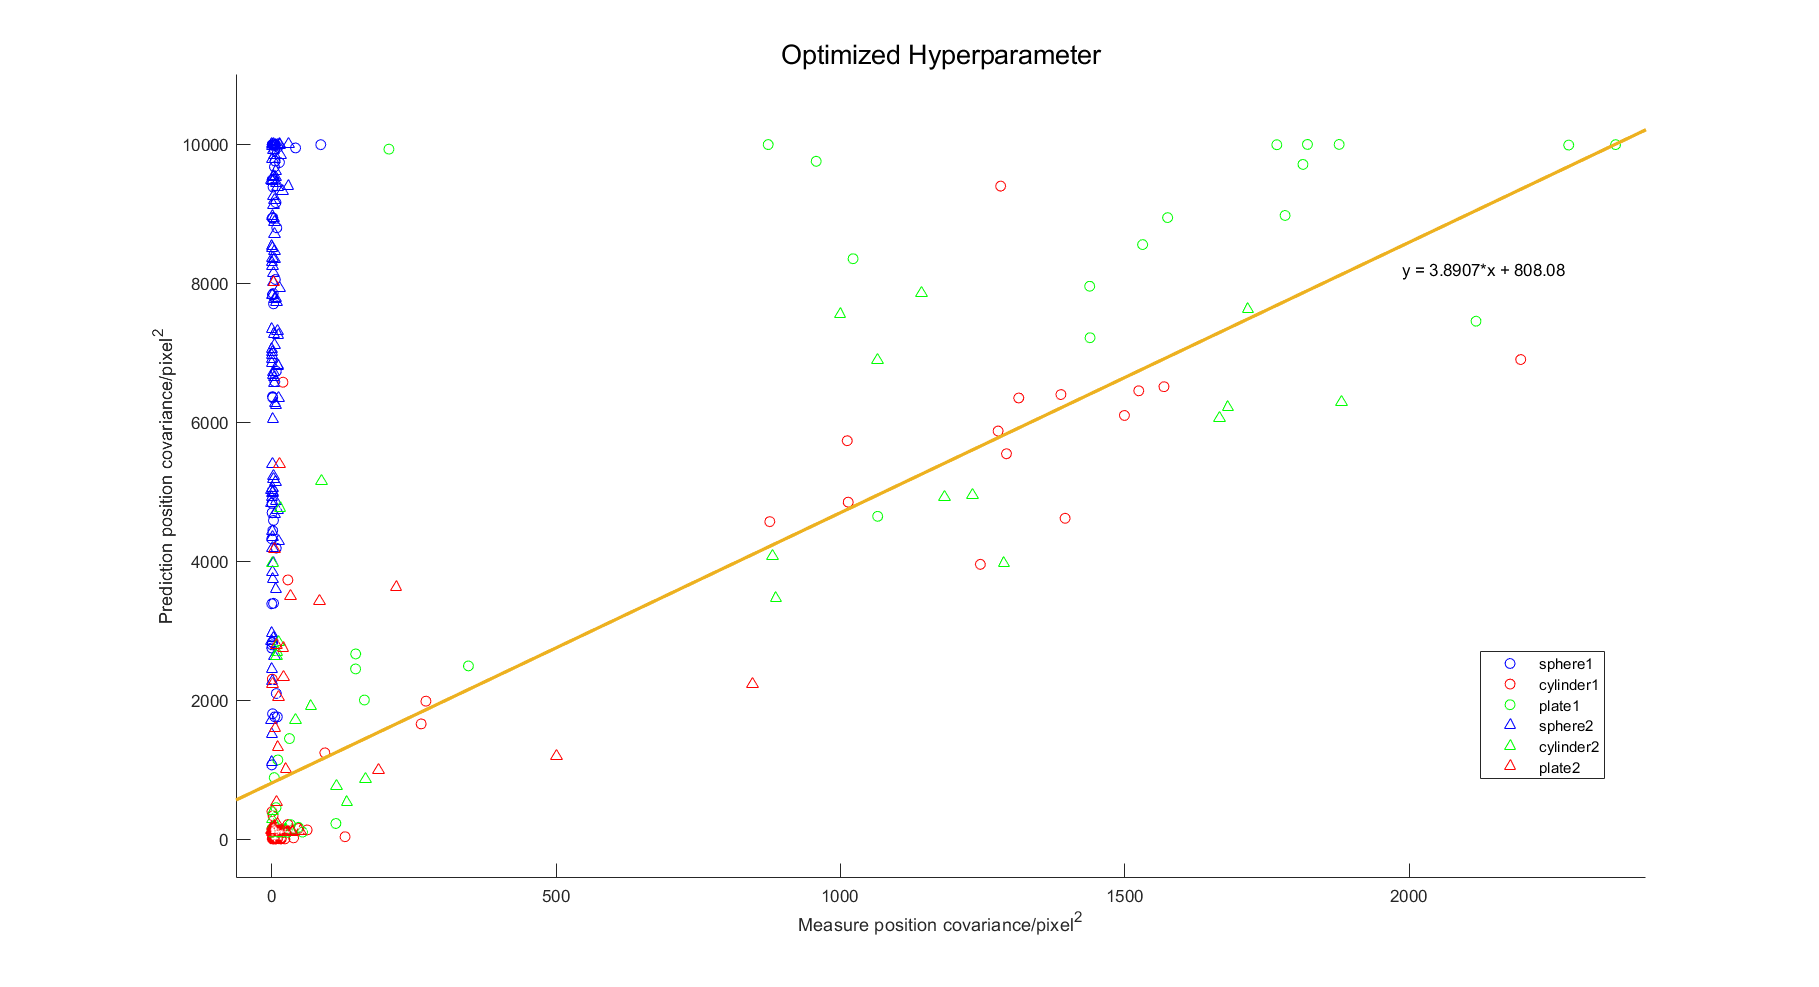
\includegraphics[width=0.9\textwidth]{figures/KF/opt-linear.png}
\caption{Optimization results with the CVA model}
\label{opt cva}
\end{figure}

\begin{figure}[htbp]
\centering
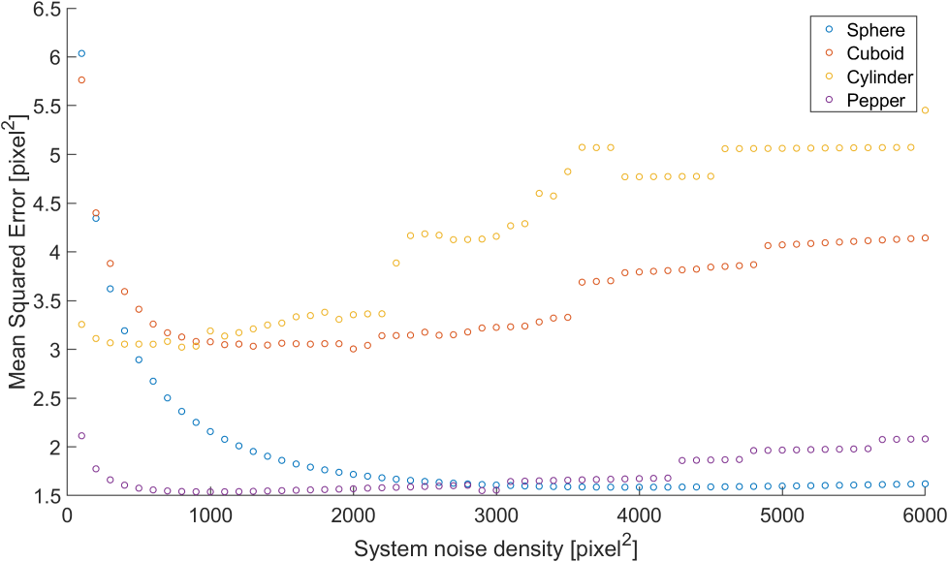
\includegraphics[width=0.9\textwidth]{figures/KF/CV result.png}
\caption{Optimization results with the CV model}
\label{opt cv}
\end{figure}


\section{Clustering and Mapping}

Try to make clusters between different datasets. Make plots showing results from different datasets. The results from different datasets are similar within the same datasets and different between different datasets, showing the different materials applies for different hyperparameters. After that give some analysis or assumption of the reason causing these difference between the datasets. 

\begin{figure}[htbp]
\centering
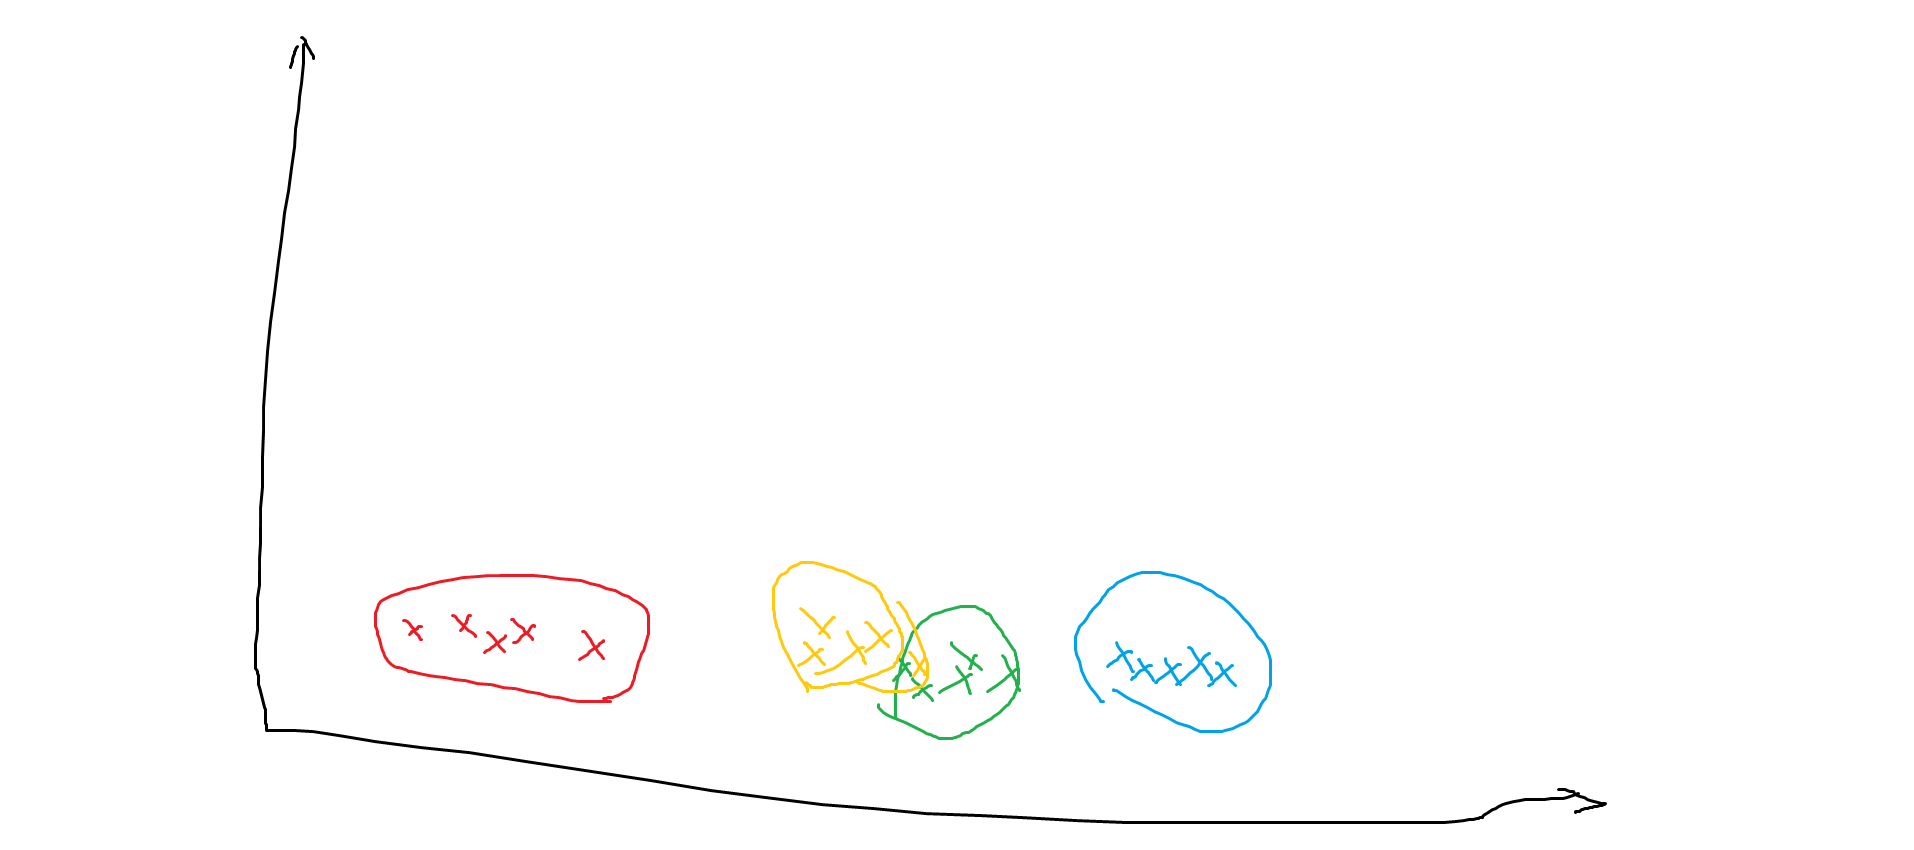
\includegraphics[width=0.9\textwidth]{figures/KF/sample cluster.png}
\caption{A sample for clustering}
\label{cluster1}
\end{figure}

\begin{figure}[htbp]
\centering
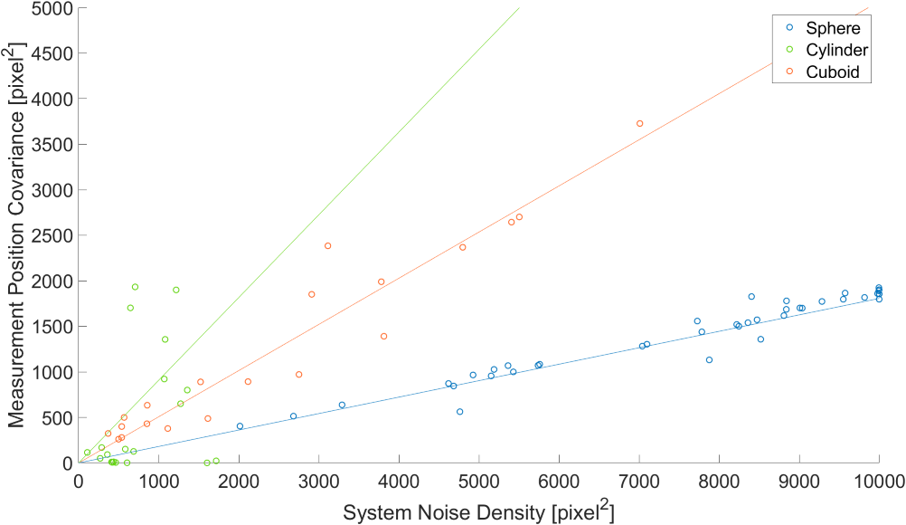
\includegraphics[width=0.9\textwidth]{figures/KF/CV result cluster.png}
\caption{Another sample for clustering}
\label{cluster2}
\end{figure}


\section{Test of Mixed Materials}

Try to make clusters between different datasets with different mix ratios.


